\section{Performance Evaluation}
\label{sec:expr}

We empirically evaluate A3Log on Amazon EC2. We will show the comparison results with other systems, with different algorithms, and with different datasets. More experimental results can be found in Appendix Sec. \ref{sec:app:expr}, including scaling performance and effectiveness of aggregations.



\subsection{Comparison to Other Systems}
\label{sec:expr:othersystems}

\noindent\textbf{Competitors}
A3Log is compared with four state-of-the-art parallel/distributed frameworks. \textbf{SociaLite} \cite{Lam:2013:SDE:2510649.2511289,Seo:2013:DSD:2556549.2556572} is a Datalog implementation for social network analysis. \textbf{Myria} \cite{Halperin:2014:DMB:2588555.2594530,Wang:2015:AFR:2824032.2824052} supports Datalog asynchronous evaluation. Both SociaLite and Myria support monotonic aggregation inside recursion. \textbf{GraphLab} \cite{Low:2012:DGF:2212351.2212354} is a graph-based parallel/distributed engine supporting asynchronous iteration. \textbf{Maiter} \cite{maiter} supports delta-based accumulative iterative computation (similar to monotonic aggregation) which can be executed asynchronously. All these systems are configured with their default parameters. Myria, GraphLab, and Maiter are configured to run with asynchronous model unless particularly mentioned. The runtime results are the execution time excluding data loading time, and each is a mean of two runs.

\noindent\textbf{Algorithms and Datasets}
We compare A3Log with other systems in the context of three algorithms, including SSSP (Program 1), PageRank (Program 2), and Connected Components (CC, Program 3). These three algorithms are all supported by these systems. For SSSP and CC, the computations terminate as soon as no new update is found. For PageRank in A3Log and Maiter, which has no notion of iterations, the computation terminates when the sum of difference to the theoretical convergence point \cite{Zhang:2011:PDF:2038916.2038929} is less than $10^{-4}$ (see Appendix Sec. \ref{sec:expr:aggregations}), based on which we know the number of iterations that is required to reach the same point (42 iterations) \cite{Zhang:2011:PDF:2038916.2038929}. Socialite and Myria (Myria does not support asynchronous PageRank) are set to run 42 iterations. GraphLab terminates after the PageRank value of every vertex changes by less than a user-specified threshold $\epsilon$ between two consecutive executions of that vertex. These algorithms are performed on a large graph dataset ClueWeb09 \cite{clueweb}. In order to finish the experiments in a reasonable time, we truncate the original dataset into a smaller ClueWeb20M dataset with 20,000,000 nodes, 243,063,334 edges, and 3.8GB size. Since ClueWeb is an unweighted graph, we assign a random weight to each edge for SSSP computation.

\begin{figure}[!t]
	\vspace{-0.1in}
	\centering
	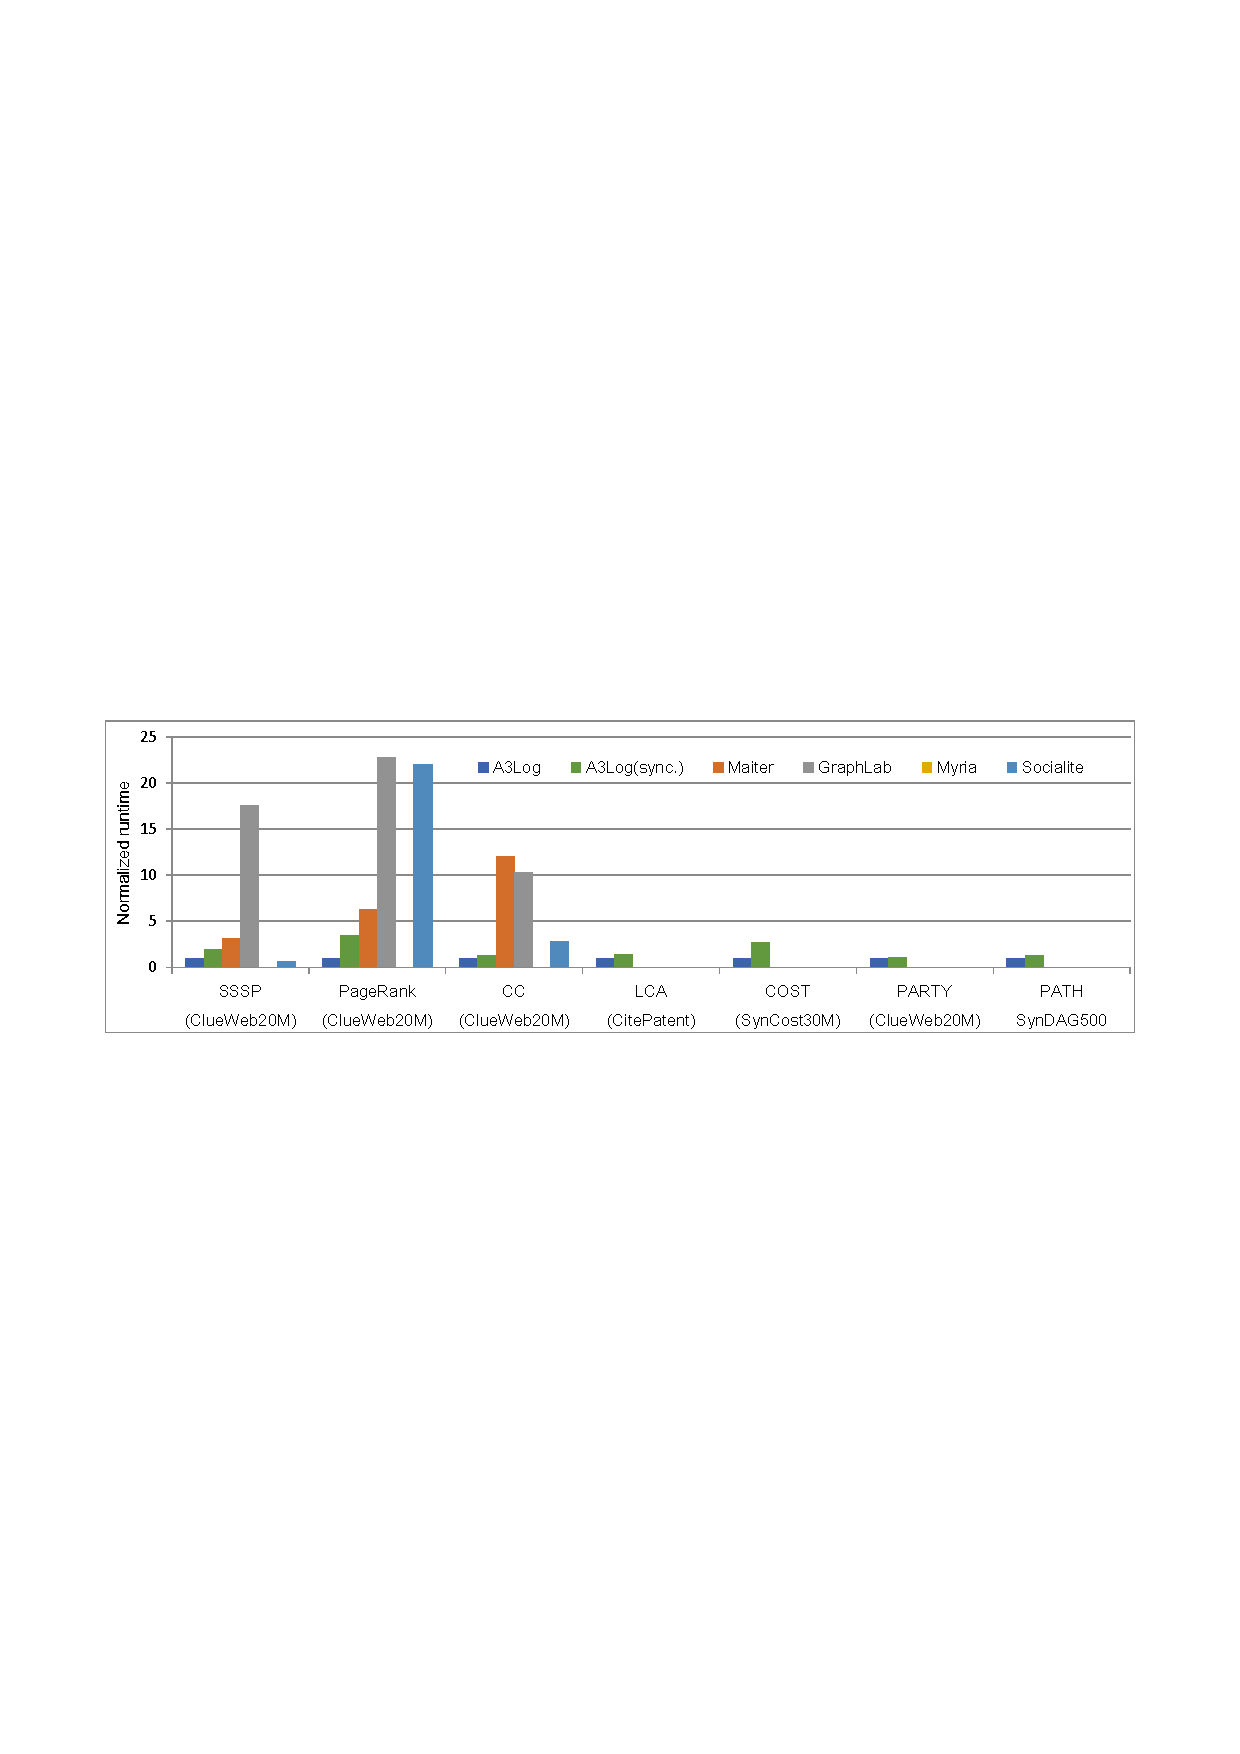
\includegraphics[width=3in]{fig/single-result}
	\vspace{-0.1in}
	\caption{Performance comparison with other systems (many-core environment)}
	\label{fig:single-result}
	\vspace{0.0in}
\end{figure}

In the shared-memory experiment, we run all the systems on an r3.8xlarge EC2 instance with 32 vCPUs and 244GB memory. We configured all these systems with 32 threads. The normalized runtime results. In general, A3Log outperforms all the competitors. For the PageRank computation, A3Log achieves 22.8X speedup over GraphLab, 22X speedup over Socialite, 6X speedup over Maiter, and much more speedup over Myria\footnote{The runtime results of Myria may be wrong because they are all unexpected long, say 135 times longer for PageRank and 321 times longer for SSSP than A3Log. We are contacting with Myria authors to fix it but cannot find the problem before the submission.} are shown in Fig. \ref{fig:single-result}. There is an exception for SSSP computation. Socialite is 1.6X faster than A3Log. This may be due to their \emph{prioritization} optimization, which is similar to our scheduling technique that leads to Dijkstra algorithm.

\begin{figure}[!t]
	\vspace{0.0in}
	\centering
	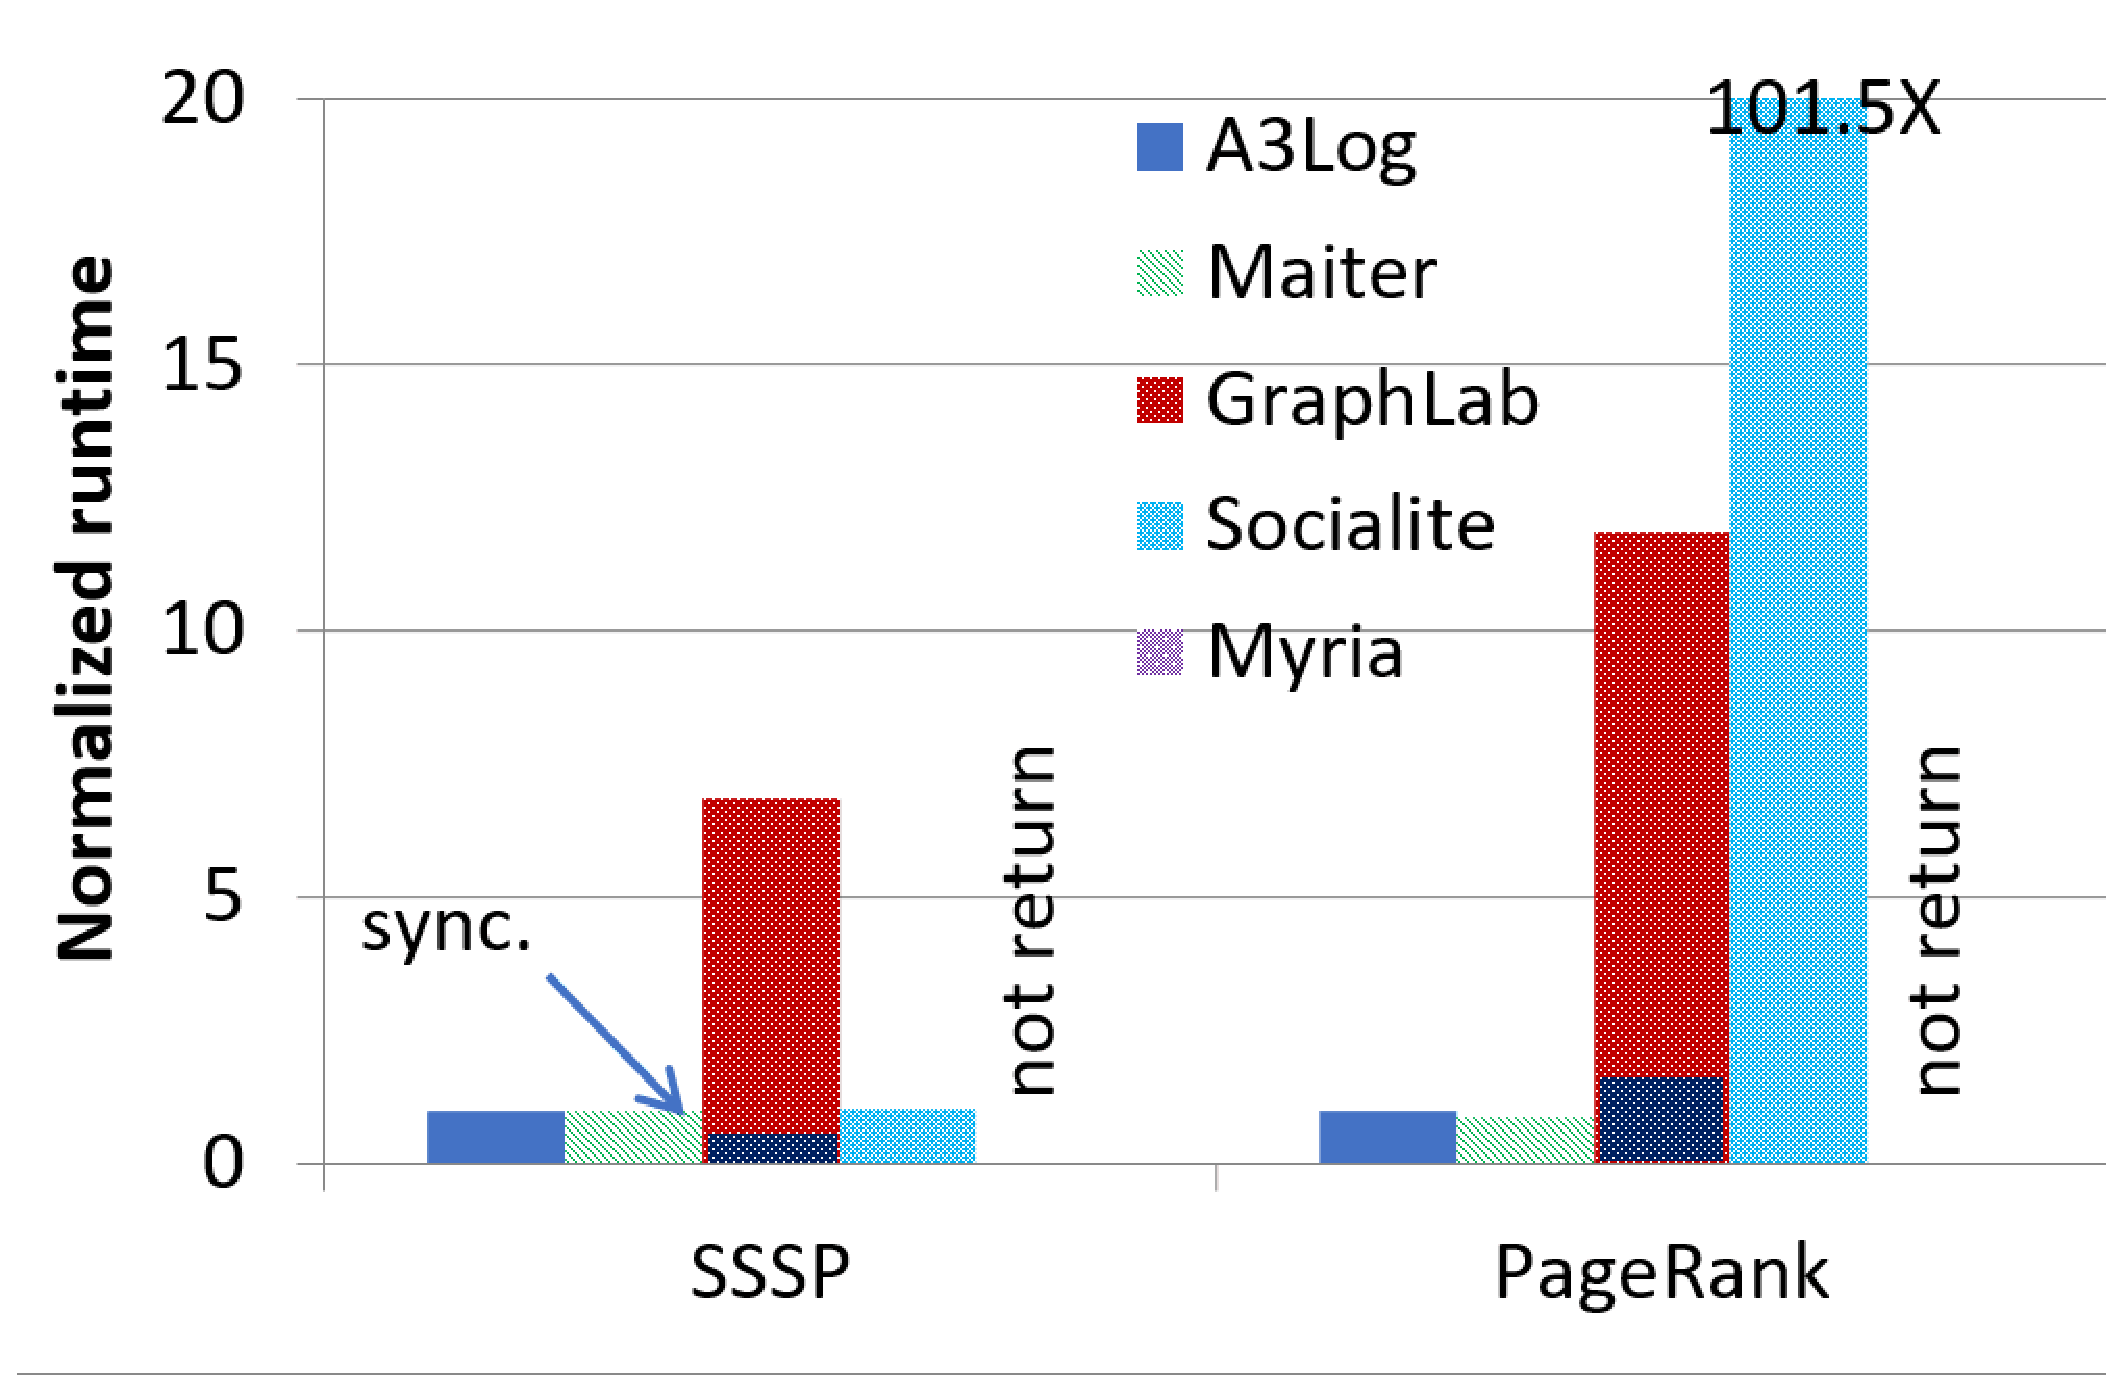
\includegraphics[width=2.4in]{fig/dist-result}
	\vspace{-0.1in}
	\caption{Performance comparison with other systems (distributed environment)}
	\label{fig:dist-result}
	\vspace{-0.2in}
\end{figure}

In the distributed experiment, we deploy all the systems on an EC2 cluster with 64 c4.2xlarge EC2 instances, each with 8 vCPUs and 15GB memory. The network bandwidth between instance workers is 10Gb/s\footnote{The network specification does not clearly describe the bandwidth but is only classified as \emph{High}, which is estimated as 10Gb/s.}. We configured all these systems with 8 threads for each worker. The normalized runtime results of SSSP and PageRank are shown in Fig. \ref{fig:dist-result}. A3Log outperforms GraphLab and Socialite on PageRank computation. The synchronous version of GraphLab performs much better than asynchronous GraphLab, which is due to its costly distributed locking \cite{Han:2015:GUB:2777598.2777604,Low:2012:DGF:2212351.2212354}. Socialite performs SSSP faster. The distributed Myria runs unexpected long without returning results, say 9 hours for PageRank and did not return. The performance of A3Log and Maiter is comparable on these two applications. The reason why A3Log does not show significant better performance in distributed environment is because of the expensive communication overhead. The communication module relies on a pure Java implementation of MPI, MPJ express \cite{mpich}, which shows about 10 times lower performance than native C implementation of Open MPI \cite{mpjperformance}. We adopt MPJ for its good compatibility but at the expense of performance. We are implementing an alternative distributed runtime based on Open MPI \cite{openmpi}.
\begin{comment}
\subsection{Performance Gain Analysis}
\label{sec:expr:optimizations}

\begin{figure}[!t]
\vspace{-0.1in}
	\centering
	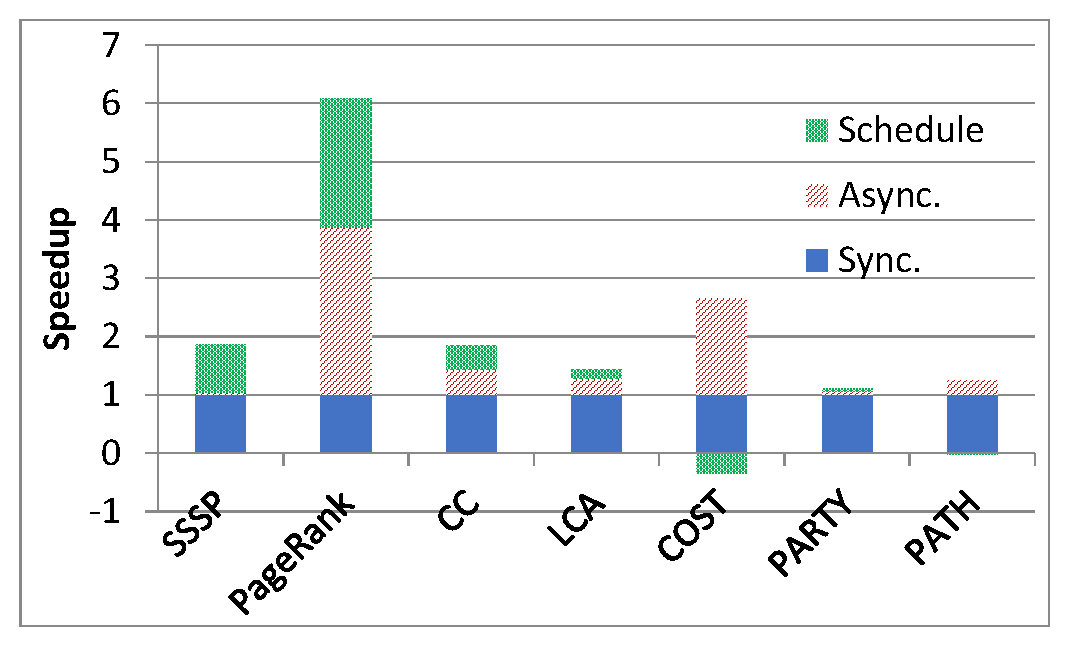
\includegraphics[width=2.8in]{fig/single-optimize}
	\caption{Performance gain analysis}
	\label{fig:single-optimize}
	\vspace{-0.0in}
\end{figure}

\begin{table*}[!t]
	%\vspace{-0.1in}
	\caption{Performance when varying workloads (shared-memory runtime, $d$ is diameter, $e$ is powerlaw exponent)}
	\vspace{-0.1in}
	\label{tab:wrokload}
	\centering
	\small
	\begin{tabular}{c|c|c|c|c|c|c|c|c|c|c|c}
		\hline
		\multirow{2}{*}{\textbf{Dataset}} & \multirow{2}{*}{\tabincell{c}{\textbf{Nodes}}} & \multirow{2}{*}{\tabincell{c}{\textbf{Edges}}} & \multirow{2}{*}{\tabincell{c}{\textbf{Graph}\\ \textbf{type}}} & \multirow{2}{*}{\tabincell{c}{\textbf{$d$}}}& \multirow{2}{*}{\tabincell{c}{\textbf{$e$}}} & \multicolumn{3}{|c}{\textbf{SSSP}} & \multicolumn{3}{|c}{\textbf{PageRank}} \\
		\cline{7-12}
		&  & & & & & \textbf{Sync.} & \textbf{Async.} & \footnotesize{\textbf{Speedup}} & \textbf{Sync.} & \textbf{Async.} & \footnotesize{\textbf{Speedup}}\\
		\hline\hline
		\textbf{Actor} & 382,219 & 33,115,812 & \footnotesize{collaborate} & 13 & 2.131 & 34.62s & 1.54s & 22.44X & 63.62s & 7.03s & 9.05X \\
		\hline
		\textbf{Amazon} & 403,394 & 3,387,388 & \footnotesize{co-purchase} & 25 & 3.151 & 79.18s & 1.55s & 51.05X & 53.77s & 1.02s & 52.9X \\
		\hline
		\textbf{arXiv} & 28,093 & 4,596,803 & co-author & 9 & 1.731 & 19.7s & 1.51s & 13.03X & 53.2s & 1.01s & 52.7X \\
		\hline
		\textbf{DBLP} & 1,314,050 & 18,986,618 & co-author & 24 & 3.221 & 55.38s & 3.18s & 17.41X & 89.76s & 5.06s & 17.75X \\
		\hline
		\textbf{Flicker} & 2,302,925 & 33,140,017 & social & 23 & 1.711 & 38.3s & 3.95s & 9.71X & 84.24s & 24.2s & 3.48X \\
		\hline
		\textbf{Livejournal} & 5,204,176 & 49,174,464 & social & 23 & 1.537 & 57.26s & 9.41s & 6.08X & 111.09s & 49.43s & \textcolor{blue}{\textbf{2.25X}} \\
		\hline
		\textbf{Orkut} & 3,072,441 & 117,184,899 & social & 10 & 1.272 & 58.99s & 14.07s & \textcolor{blue}{\textbf{4.19X}} & 187.74s & 16.18s & 11.6X \\
		\hline
		\textbf{Patent-US} & 3,774,768 & 16,518,947 & citation & 26 & 4.001 & 66.83s & 3.21s & 20.8X & 68.06s & 6.11s & 11.15X \\
		\hline
		\textbf{Prosper} & 89,269 & 3,394,979 & loan & 8 & 2.191 & 37.75s & 1.51s & 24.93X & 52.61s & 1.02s & 51.58X \\
		\hline
		\textbf{RoadCA} & 1,965,206 & 2,766,607 & road net & 865 & 8.991 & 140.43s & 1.55s & 90.31X & 57.06s & 1.03s & \textcolor{red}{\textbf{55.59X}} \\
		\hline
		\textbf{RoadTX} & 1,379,917 & 1,921,660 & road net & 1064 & 8.901 & 137.2s & 1.55s & 88.4X & 54.49s & 1.02s & 53.63X \\
		\hline
		\textbf{Skitter} & 1,696,415 & 11,095,298 & Internet & 31 & 2.291 & 31.09s & 1.55s & 20.01X & 59.51s & 3.04s & 19.56X \\
		\hline
		\textbf{soc-LiveJ} & 4,847,571 & 68,475,391 & social & 20 & 2.651 & 67.2s & 11.2s & 6X & 113.51s & 39.2s & 2.9X \\
		\hline
		\textbf{soc-Pokec} & 1,632,803 & 30,622,564 & social & 14 & 3.081 & 53.85s & 4.81s & 11.19X & 76.83s & 15.1s & 5.09X \\
		\hline
		\textbf{TREC} & 1,601,787 & 8,063,026 & web & 112 & 2.231 & 130.84s & 1.6s & 81.62X & 55.29s & 2.03s & 27.23X \\
		\hline
		\textbf{\footnotesize{web-BerkStan}} & 685,230 & 7,600,595 & web & 208 & 2.601 & 692.08s & 3.1s & \textcolor{red}{\textbf{222.82X}} & 54.13s & 2.02s & 26.76X \\
		\hline
		\textbf{web-Google} & 875,713 & 5,105,039 & web & 24 & 2.731 & 70.8s & 1.59s & 44.64X & 54.24s & 2.03s & 26.67X \\
		\hline
		\textbf{Wiki-Talk} & 2,987,535 & 24,981,163 & \footnotesize{communicate} & 9 & 1.811 & 23.81s & 3.1s & 7.68X & 83.57s & 28.27s & 2.96X \\
		\hline
		\textbf{Youtube-u} & 3,223,589  & 9,375,374 & social & 31 & 2.211 & 30.6s & 2.43s & 12.6X & 65.91s & 5.08s & 12.96X \\
		\hline
		\textbf{\footnotesize{Zhishi-Baidu}} & 2,141,300 & 17,794,839 & web & 20 & 2.291 & 49.19s & 3.29s & 14.96X & 66.72s & 8.09s & 8.25X\\
		\hline
	\end{tabular}
	\vspace{-0.1in}
\end{table*}
\end{comment}
In order to analyze the factors for performance improvement and eliminate the interference from system implementation factors, we also implement a synchronous version of A3Log, which uses synchronous semi-naive evaluation (i.e., synchronous accumulated recursive programs). In addition, we turn off the scheduling then it shows the performance ahieved by pure asynchronous aggregation.

\noindent\textbf{Algorithms and Datasets}
We test more algorithms to see the effect variations on different workloads, including Least Common Ancestor (LCA, Program 6), ``What is the cost of each part?'' (COST, Program 7), ``Who will come to the party?'' (PARTY, Program 9), and ``Computing Paths in a DAG'' (PATH, Program 4). More details of these algorithms can be found in Appendix Sec. \ref{sec:app:example}. For LCA, we use a citation network Patent-US \cite{konect}. For COST, we synthetically generate a hierarchical (tree-like) dataset with 30,000,000 tree nodes. PARTY is a graph based algorithm, so we use the same ClueWeb20M dataset. For PATH, we synthetically generate a directed acyclic graph (DAG) dataset with 500 nodes and 35,952 edges. PATH is a computation intensive workload since it evaluates the paths between all pairs.


We run these algorithms on the an r3.8xlarge EC2 instance with 32 vCPUs and 244GB memory. All these experiments are run with 32 threads. Fig. \ref{fig:single-optimize} shows the results. The runtime by synchronous semi-naive evaluation is considered as the baseline. The speedups from asynchronous execution and prioritized scheduling exhibit variations for different workloads. Generally speaking, the graph based algorithms benefit from asynchronous aggregation and priority scheduling more. For SSSP and PageRank, great performance gains are achieved by priority scheduling. However, for COST, the priority scheduling brings negative effect. This is because that COST aims to compute all parts' cost in a hierarchical structure and the computations on these parts equally contribute to the output. Using priority scheduling will not bring any benefit but only incurs scheduling overhead. However, we still take advantage of asynchronous aggregation to avoid synchronizations and achieve better performance.
 \subsection{Scaling Performance}
 \label{sec:expr:scale}
 
 \begin{figure}[!t]
 	\centering
 	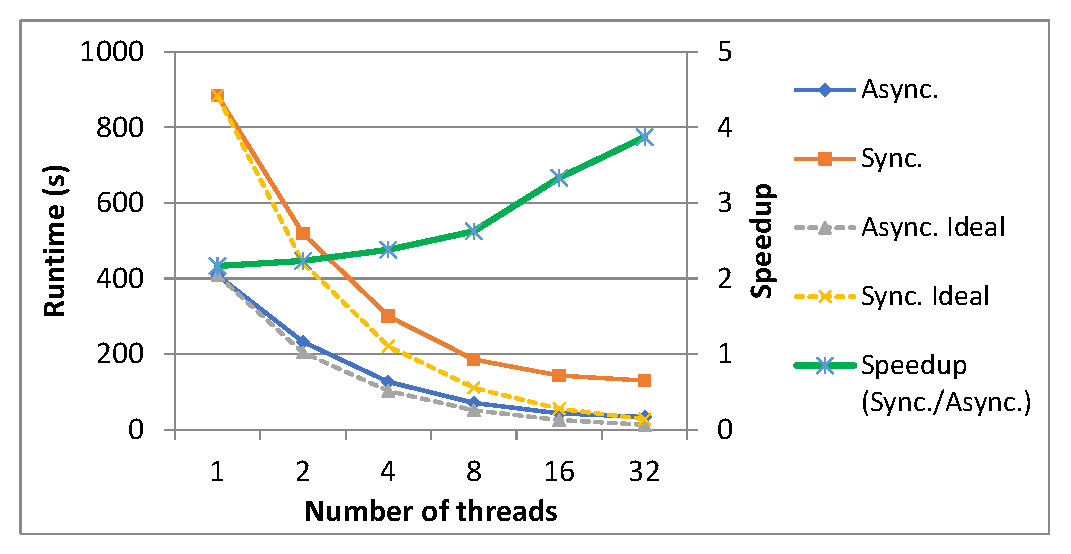
\includegraphics[width=2.8in]{fig/single-scalability}
 	\vspace{-0.1in}
 	\caption{Scaling performance (many-core)}
 	\label{fig:single-scalability}
 \end{figure}
 
 \begin{figure}[!t]
 	\centering
 	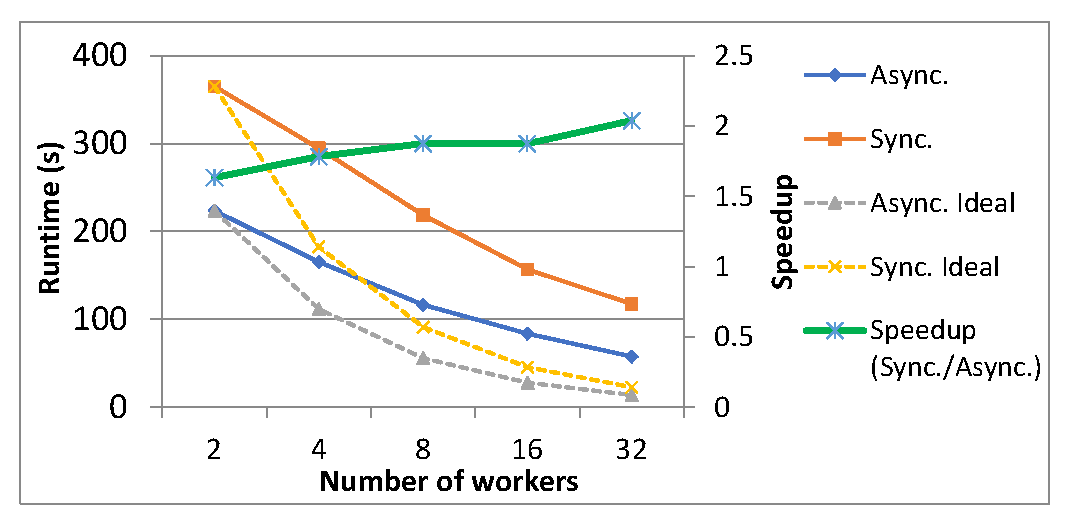
\includegraphics[width=2.8in]{fig/dist-scalability}
 	\vspace{-0.1in}
 	\caption{Scaling performance (distributed)}
 	\label{fig:dist-scalability}
 \end{figure}
 
 
asynchronous aggregation is expected to achieve better scaling performance. We evaluate the scaling performance of A3Log's share-memory runtime on an r3.8xlarge EC2 instance. We perform PageRank computation with the synchronous and asynchronous versions (without scheduling) of A3Log and vary the number of threads from 1 to 32. The runtime results are shown in Fig. \ref{fig:single-scalability}. We also draw the ideal scaling performance curve based on the runtime result of 1 thread. The asynchronous A3Log's scaling performance curve is closer to its ideal curve, while the synchronous A3Log exhibits larger difference to its ideal curve when running on more threads. Asynchronous execution also shows higher speedup over synchronous execution when running on more threads.
 
 We also evaluate the scaling performance of A3Log's distributed runtime on a cluster with a number of c4.large EC2 instances, each with 2 vCPUs and 3.75GB memory. We perform PageRank computation with the synchronous and asynchronous executions (without scheduling) and vary the number of workers from 1 to 32. The runtime results are shown in Fig. \ref{fig:dist-scalability}. We also draw the ideal scaling performance curve based on the runtime result of 2-workers. Similar to the results on shared-memory runtime, asynchronous execution also shows better scaling performance. Higher speedup over synchronous execution is achieved when running on larger size cluster.


\subsection{Comparison with Different Workloads}
\label{sec:expr:workloads}
{\color{red}Here I wanna add something about Partition sensitive}
To see the performance when varying datasets, we choose 20 various graph datasets with various graph structures and various graph properties. All the datasets are downloaded from \cite{konect}. We use two typical graph algorithms SSSP and PageRank for evaluation. We run the shared-memory version of A3Log on a c4-2xlarge EC2 instance with 8 vCPU and 60GB memory. A3Log is configured with 8 threads. We compare the algorithm runtime of synchronous execution and asynchronous execution on these graphs.

Table \ref{tab:wrokload} shows the graph datasets and the runtime results. The asynchronous execution exhibits 4.19X-222.82X speedup over synchronous execution on SSSP computation, and 2.25X-55.59X speedup over synchronous execution on PageRank computation. Generally speaking, asynchronous SSSP achieves higher speedup on large diameter graphs, and asynchronous PageRank computation achieves higher speedup on the graphs with larger powerlaw exponent. Of course, the performance speedup also relates to the graph structures and graph types. Note that, in asynchronous execution, the termination check is performed periodically (every 1 second in this experiment). If the runtime results of asynchronous executions shows 1.x second, they may converge less than 1 second. Thus, the performance of asynchronous execution is expected to be even higher.

